%%%%%%%%%%%%%%%%%%%%%%%%%%%%%%%%%%%%%%%%%
% Masters/Doctoral Thesis 
% LaTeX Template
% Version 2.4 (22/11/16)
%
% This template has been downloaded from:
% http://www.LaTeXTemplates.com
%
% Version 2.x major modifications by:
% Vel (vel@latextemplates.com)
%
% This template is based on a template by:
% Steve Gunn (http://users.ecs.soton.ac.uk/srg/softwaretools/document/templates/)
% Sunil Patel (http://www.sunilpatel.co.uk/thesis-template/)
%
% Template license:
% CC BY-NC-SA 3.0 (http://creativecommons.org/licenses/by-nc-sa/3.0/)
%
%%%%%%%%%%%%%%%%%%%%%%%%%%%%%%%%%%%%%%%%%

%----------------------------------------------------------------------------------------
%	PACKAGES AND OTHER DOCUMENT CONFIGURATIONS
%----------------------------------------------------------------------------------------

\documentclass[
11pt, % The default document font size, options: 10pt, 11pt, 12pt
%oneside, % Two side (alternating margins) for binding by default, uncomment to switch to one side
english, % ngerman for German
onehalfspacing, % Single line spacing, alternatives: singlespacing, onehalfspacing or doublespacing
%draft, % Uncomment to enable draft mode (no pictures, no links, overfull hboxes indicated)
%nolistspacing, % If the document is onehalfspacing or doublespacing, uncomment this to set spacing in lists to single
%liststotoc, % Uncomment to add the list of figures/tables/etc to the table of contents
%toctotoc, % Uncomment to add the main table of contents to the table of contents
%parskip, % Uncomment to add space between paragraphs
%nohyperref, % Uncomment to not load the hyperref package
headsepline, % Uncomment to get a line under the header
%chapterinoneline, % Uncomment to place the chapter title next to the number on one line
%consistentlayout, % Uncomment to change the layout of the declaration, abstract and acknowledgements pages to match the default layout
]{MastersDoctoralThesis} % The class file specifying the document structure

\usepackage[utf8]{inputenc} % Required for inputting international characters
\usepackage[T1]{fontenc} % Output font encoding for international characters

\usepackage{palatino} % Use the Palatino font by default
\usepackage[square,numbers]{natbib}
\usepackage{multicol,graphicx}
\usepackage{subcaption}



\usepackage[autostyle=true]{csquotes}
\graphicspath{ {Figures/} }
%----------------------------------------------------------------------------------------
%	MARGIN SETTINGS
%----------------------------------------------------------------------------------------

\geometry{
	paper=a4paper, % Change to letterpaper for US letter
	inner=2.5cm, % Inner margin
	outer=3.8cm, % Outer margin
	bindingoffset=.5cm, % Binding offset
	top=1.5cm, % Top margin
	bottom=1.5cm, % Bottom margin
	%showframe, % Uncomment to show how the type block is set on the page
}

%----------------------------------------------------------------------------------------
%	THESIS INFORMATION
%----------------------------------------------------------------------------------------

\thesistitle{Thesis 22 Title} % Your thesis title, this is used in the title and abstract, print it elsewhere with \ttitle
\supervisor{Dr. James \textsc{Smith}} % Your supervisor's name, this is used in the title page, print it elsewhere with \supname
\examiner{} % Your examiner's name, this is not currently used anywhere in the template, print it elsewhere with \examname
\degree{Doctor of Philosophy} % Your degree name, this is used in the title page and abstract, print it elsewhere with \degreename
\author{John \textsc{Smith}} % Your name, this is used in the title page and abstract, print it elsewhere with \authorname
\addresses{} % Your address, this is not currently used anywhere in the template, print it elsewhere with \addressname

\subject{Biological Sciences} % Your subject area, this is not currently used anywhere in the template, print it elsewhere with \subjectname
\keywords{} % Keywords for your thesis, this is not currently used anywhere in the template, print it elsewhere with \keywordnames
\university{\href{http://www.university.com}{University Name}} % Your university's name and URL, this is used in the title page and abstract, print it elsewhere with \univname
\department{\href{http://department.university.com}{Department or School Name}} % Your department's name and URL, this is used in the title page and abstract, print it elsewhere with \deptname
\group{\href{http://researchgroup.university.com}{Research Group Name}} % Your research group's name and URL, this is used in the title page, print it elsewhere with \groupname
\faculty{\href{http://faculty.university.com}{Faculty Name}} % Your faculty's name and URL, this is used in the title page and abstract, print it elsewhere with \facname

\AtBeginDocument{
\hypersetup{pdftitle=\ttitle} % Set the PDF's title to your title
\hypersetup{pdfauthor=\authorname} % Set the PDF's author to your name
\hypersetup{pdfkeywords=\keywordnames} % Set the PDF's keywords to your keywords
}

\begin{document}

\frontmatter % Use roman page numbering style (i, ii, iii, iv...) for the pre-content pages

\pagestyle{plain} % Default to the plain heading style until the thesis style is called for the body content

%----------------------------------------------------------------------------------------
%	TITLE PAGE
%----------------------------------------------------------------------------------------

\begin{titlepage}
\begin{center}

\vspace*{.06\textheight}
{\scshape\LARGE \univname\par}\vspace{1.5cm} % University name
\textsc{\Large Doctoral Thesis}\\[0.5cm] % Thesis type

\HRule \\[0.4cm] % Horizontal line
{\huge \bfseries \ttitle\par}\vspace{0.4cm} % Thesis title
\HRule \\[1.5cm] % Horizontal line
 
\begin{minipage}[t]{0.4\textwidth}
\begin{flushleft} \large
\emph{Author:}\\
\href{http://www.johnsmith.com}{\authorname} % Author name - remove the \href bracket to remove the link
\end{flushleft}
\end{minipage}
\begin{minipage}[t]{0.4\textwidth}
\begin{flushright} \large
\emph{Supervisor:} \\
\href{http://www.jamessmith.com}{\supname} % Supervisor name - remove the \href bracket to remove the link  
\end{flushright}
\end{minipage}\\[3cm]
 
\vfill

\large \textit{A thesis submitted in fulfillment of the requirements\\ for the degree of \degreename}\\[0.3cm] % University requirement text
\textit{in the}\\[0.4cm]
\groupname\\\deptname\\[2cm] % Research group name and department name
 
\vfill

{\large \today}\\[4cm] % Date
%\includegraphics{Logo} % University/department logo - uncomment to place it
 
\vfill
\end{center}
\end{titlepage}

%----------------------------------------------------------------------------------------
%	DECLARATION PAGE
%----------------------------------------------------------------------------------------

\begin{declaration}
\addchaptertocentry{\authorshipname} % Add the declaration to the table of contents
\noindent I, \authorname, declare that this thesis titled, \enquote{\ttitle} and the work presented in it are my own. I confirm that:

\begin{itemize} 
\item This work was done wholly or mainly while in candidature for a research degree at this University.
\item Where any part of this thesis has previously been submitted for a degree or any other qualification at this University or any other institution, this has been clearly stated.
\item Where I have consulted the published work of others, this is always clearly attributed.
\item Where I have quoted from the work of others, the source is always given. With the exception of such quotations, this thesis is entirely my own work.
\item I have acknowledged all main sources of help.
\item Where the thesis is based on work done by myself jointly with others, I have made clear exactly what was done by others and what I have contributed myself.\\
\end{itemize}
 
\noindent Signed:\\
\rule[0.5em]{25em}{0.5pt} % This prints a line for the signature
 
\noindent Date:\\
\rule[0.5em]{25em}{0.5pt} % This prints a line to write the date
\end{declaration}
%----------------------------------------------------------------------------------------
%	ABSTRACT PAGE
%----------------------------------------------------------------------------------------
\begin{abstract}
\addchaptertocentry{\abstractname} P300-based spellers are one of the main methods for EEG-based brain-computer interface, and the detection of the P300 target event with high accuracy is an important prerequisite. The rapid serial visual presentation (RSVP) protocol is of high interest because it can be used by patients who have lost control over their eyes. In this study we wish to explore the suitability of recurrent neural networks (RNNs) as a machine learning method for identifying the P300 signal in RSVP data. We systematically compare RNN with alternative methods such as linear discriminant analysis (LDA) and convolutional neural network (CNN). Our results indicate that RNN shows good results only with large amounts of data, and we show that a network combining CNN and RNN is significantly more resilient to temporal noise than other methods.
\end{abstract}
%----------------------------------------------------------------------------------------
%	ACKNOWLEDGEMENTS
%----------------------------------------------------------------------------------------
\begin{acknowledgements}
\addchaptertocentry{\acknowledgementname} % Add the acknowledgements to the table of contents
The acknowledgments and the people to thank go here, don't forget to include your project advisor\ldots
\end{acknowledgements}

%----------------------------------------------------------------------------------------
%	LIST OF CONTENTS/FIGURES/TABLES PAGES
%----------------------------------------------------------------------------------------

\tableofcontents % Prints the main table of contents

\listoffigures % Prints the list of figures

\listoftables % Prints the list of tables

%----------------------------------------------------------------------------------------
%	ABBREVIATIONS
%----------------------------------------------------------------------------------------

\begin{abbreviations}{ll} % Include a list of abbreviations (a table of two columns)

\textbf{LAH} & \textbf{L}ist \textbf{A}bbreviations \textbf{H}ere\\
\textbf{WSF} & \textbf{W}hat (it) \textbf{S}tands \textbf{F}or\\

\end{abbreviations}

%----------------------------------------------------------------------------------------
%	PHYSICAL CONSTANTS/OTHER DEFINITIONS
%----------------------------------------------------------------------------------------

\begin{constants}{lr@{${}={}$}l} % The list of physical constants is a three column table

% The \SI{}{} command is provided by the siunitx package, see its documentation for instructions on how to use it

Speed of Light & $c_{0}$ & \SI{2.99792458e8}{\meter\per\second} (exact)\\
%Constant Name & $Symbol$ & $Constant Value$ with units\\

\end{constants}

%----------------------------------------------------------------------------------------
%	SYMBOLS
%----------------------------------------------------------------------------------------

\begin{symbols}{lll} % Include a list of Symbols (a three column table)

$a$ & distance & \si{\meter} \\
$P$ & power & \si{\watt} (\si{\joule\per\second}) \\
%Symbol & Name & Unit \\

\addlinespace % Gap to separate the Roman symbols from the Greek

$\omega$ & angular frequency & \si{\radian} \\

\end{symbols}

%----------------------------------------------------------------------------------------
%	DEDICATION
%----------------------------------------------------------------------------------------

\dedicatory{For/Dedicated to/To my\ldots} 

%----------------------------------------------------------------------------------------
%	THESIS CONTENT - CHAPTERS
%----------------------------------------------------------------------------------------

\mainmatter % Begin numeric (1,2,3...) page numbering

\pagestyle{thesis} % Return the page headers back to the "thesis" style

% Include the chapters of the thesis as separate files from the Chapters folder
% Uncomment the lines as you write the chapters

\chapter{Introduction}
\section{INTRODUCTION}
\vspace{0.4cm}

Neural networks have recently been shown to achieve outstanding performance in several machine learning domains such as image recognition \cite{krizhevsky2012imagenet}  and voice recognition~\cite{hinton2012deep}. Most of these breakthroughs have been achieved with convolutional neural networks (CNNs)~\cite{Lenet98}, but some promising results has also been demonstrated by using recurrent neural networks (RNNs) for tasks such as speech and handwriting recognition~\cite{graves2013speech, graves2008unconstrained}, usually when using the long short-term memory (LSTM) architecture ~\cite{LSTM_origin}.

\begin{samepage}
	There have been some studies on using ``deep neural networks'' for P300 classification \cite{P300_CNN, RSVP_P300_geva}. The results reported, despite some success, do not show the same dramatic progress achieved by `deep learning' methods as compared to the previous state of the art; while in areas such as image or voice recognition `deep' neural networks have resulted in classification accuracy exceeding other methods by far, this has not yet been the case with EEG in general and P300 detection specifically. The small number of samples typically available in neuroscience (or BCI) is most likely one of the main reasons. In addition, the high dimensionality of the EEG signal, the low signal to noise (SNR) and the existence of outliers in the data, pose other difficulties when trying to use neural networks for BCI tasks (see \cite{lotte2007review}). The main question in this research is whether the RNN model, and particularly LSTM, can enhance the accuracy of P300-based BCI systems and if so, under what conditions.
\end{samepage}

\vspace{0.4cm}
\section{BACKGROUND}
\vspace{0.4cm}


P300-based BCI systems can identify when a subject's attention is distracted toward a rare event by examining the subject's electroencephalogram (EEG) data. The first system that used the P300 effect was presented by~\cite{FirstP300} and since then different versions of P300 based BCI systems were suggested. One example of such a paradigm is the P300 rapid serial visual presentation (RSVP) speller. In this paradigm letters are presented one after the other in a random order, and the subject is asked to pay attention only to one of the letters called \textit{target} letter or \textit{target stimuli} (by counting them silently, for example). Whenever a subject pays attention to the target letter, a special waveform called P300 is expected to occur when a person's attention is distracted toward a rare event. It is called P300 since there is usually a peak in the EEG amplitude 300ms after the presentation of a target event. The advantage of the RSVP paradigm is that it does not require any eye movements, and can thus be operated by patients who have lost control of their eye gaze completely.

There are a lot of methods for building systems that can identify P300 signal for a BCI task. Blankertz et al.~\cite{P300_Tutorial} suggest to select the time interval with maximal separation between the target and non target samples, average their \textit{electro-potential} value and use shrinkage LDA to classify these features. Using this method has a drawback due to the low complexity of LDA model \cite{cincotti2003comparison}. The winner of the BCI competition III: dataset II used an ensemble of support vector machines (SVM) \cite{P300SVMWinner}, and other methods include hidden Markov model, k-nearest neighbours, and more  \cite{cincotti2003comparison}.

More recently, given the success of `deep' neural networks \cite{krizhevsky2012imagenet}, there have been several attempts to apply `deep learning' for BCI related tasks. Cecotti and Graser~\cite{P300_CNN} were the first to use CNNs  for P300 speller. In their work, they train an ensemble of CNN-based P300 classifiers to identify the existence of P300. Manor and Geva~\cite{RSVP_P300_geva} used CNN for the RSVP P300 classification task and suggested a new spatio-temporal regularization which have shown improvement in the performance.


Unlike feed forward network models such as CNN and multi-layer perceptron (MLP),  the RNN architecture allows directed cycles within the network, which enable the model to ``memorize past events''. LSTM \cite{LSTM_origin} is a type of RNN, which includes a special node that can be described as a differentiable memory cell. The specific architecture of LSTM enables it to overcome some of the weakness of simple RNNs~\cite{bengio1994learning}.

There are several reasons why LSTM is a good candidate for modelling the P300 pattern. First, RNN and LSTM have shown success when modeling time series for tasks such as handwriting and speech recognition \cite{graves2013speech,  graves2008unconstrained, yue2015beyond}. Second, RNN is known to have the capability to approximate dynamical systems \cite{li2005approximation}, which makes it a natural candidate for modelling the dynamics of EEG data. Another motivation is that RNN can be seen as powerful form of hidden Markov models (HMM), which have been shown to classify EEG successfully \cite{solhjoo2005classification,obermaier2001hidden,cincotti2003comparison}; RNNs can be seen as HMMs with an exponentially large state space and an extremely compact parametrization~\cite{sutskever2009recurrent}.

LSTM was already used for analysing EEG data for emotion detection \cite{soleymani2014continuous} and a phenomena called behavioral microsleeps \cite{davidson2005detecting}. Bahshivan et al.~\cite{LSTM_EEG} modeled inter-subject EEG features for identifying cognitive load by using convolutional LSTM. They created a video from three different band powers in each electrode. One of the major differences between their work and ours is that we use the original signal without any feature extraction (such as band power), and we focus specifically on P300 speller.

\section{TODO}
\begin{itemize}
	\item algorithm long explanation
\end{itemize}

\chapter{MATERIALS AND METHODS}

We compared the performance of LSTM based methods with other methods on a dataset from a RSVP P300 speller study~\cite{BlaknertzExperiment}. We used  average prediction across 10 trials to measure the P300 speller accuracy as applied in~\cite{BlaknertzExperiment}.

The dataset includes 55 channels of EEG recordings from 11 subjects. Each subject is presented with 10 repetitions of 60 to 70 sets of 30 different letters and symbols. In total there are approximately 20,000 samples for each subject where 1/30 of them are supposed to contain a P300 wave. While the original experiment contains 3 different settings (interval of 116ms with/without colors and 83ms with color), we used the experiment setting of 116ms intervals with letters in different colors. For more detail, see \cite{BlaknertzExperiment}. 

In addition to the filters applied in~\cite{BlaknertzExperiment}, all models that we used share the same pre-processing stage of down-sampling the input frequency from 200Hz to 25 Hz. The result is that each learning sample is a matrix of 55 channels with 25 time samples each, or $55*25 = 1375$ features. Each sample thus covers exactly 1 second around the target event, at times [-200,800] ms.

The models evaluated in this experiment are:
\begin{itemize}
	\item LDA - A common method used in P300 classification for BCI is LDA \cite{BlaknertzExperiment,P300_Tutorial}. Here we will use a simplified version; unlike \cite{BlaknertzExperiment} we use all the timestamps as features, and we are using a non-shrinkage version of LDA.
	
	\item CNN (Fig.\ref{fig:CNN_model}) -- The CNN model we use is similar to the one used in \cite{P300_CNN}. The first layer is composed of 10  spatial filters, each of size $55*1$ -- the number of channels. The second layer contains 13 different temporal filters with size of $1*5$. Each one of the temporal filters processes 5 subsequent time stamps without overlapping. The third and fourth layers are simple fully connected layers followed by a single cell with sigmoid activation function that emits a scalar.
	
	\item LSTM large/small (Fig.\ref{fig:LSTM_model}) -- LSTM large/small are both composed of single LSTM layers with 100 and 30 hidden cells in each, correspondingly. Both models end with a single cell with sigmoid activation layer that emits a scalar.
	
	\item LSTM-CNN large/small Fig.\ref{fig:LSTM_model_CNN} -- The model has CNN as a first layer (the spatial domain layer) and LSTM as the second layer for the temporal domain. The first convolutional layer is the same as in the CNN model. Unlike the CNN model, the temporal layer is an LSTM layer with 100/30 hidden cells. The last layer contains a single cell a with sigmoid activation layer that emits a scalar.

\end{itemize}

	\begin{figure*}[t]
		\centering
		\begin{minipage}{.3\textwidth}
			\centering
			\begin{subfigure}{1.0\textwidth}
				\centering
				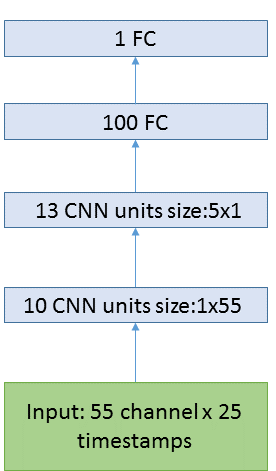
\includegraphics[height=5cm]{P300_CNN_arch}
				%	\end{center}
				\caption{CNN model}
				\label{fig:CNN_model}
			\end{subfigure}
		\end{minipage}	
		\begin{minipage}{.3\textwidth}
			
			\centering
			\begin{subfigure}{1.0\textwidth}
				\centering
				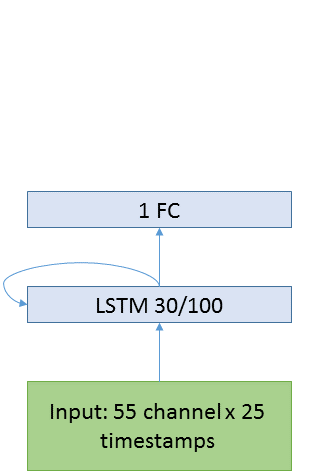
\includegraphics[height=5cm]{P300_LSTM_arch_v3}
				%	\end{center}
				\caption{LSTM model}
				\label{fig:LSTM_model}
			\end{subfigure}
			
		\end{minipage}%
		\begin{minipage}{.3\textwidth}
			\centering
			\begin{subfigure}{1.0\textwidth}
			\centering
			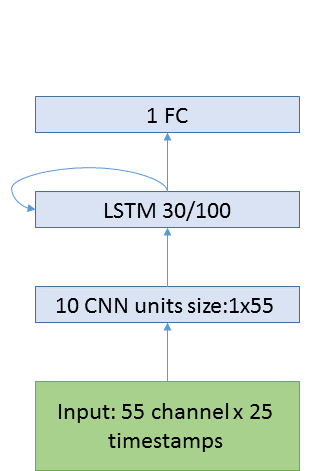
\includegraphics[height=5cm]{P300_LSTM_CNN_arch_v3}		
			%	\end{center}
			\caption{CNN-LSTM model}
			\label{fig:LSTM_model_CNN}		
			\end{subfigure}
		\end{minipage}
		
		\caption{Schematic diagrams of the neural networks evaluated. FC stands for fully connected layers.}
	\end{figure*}
								
								
In order to examine the power of each method in modelling the inter-subject and  intra-subject variance we have conducted the following experiments:
\begin{enumerate}
	\item Training and testing on each subject's data separately in order to explore intra-subject generalization.
	\item Training and testing on all the different subjects data combined in order to investigate the impact of larger amounts of data.
	\item Training on all subjects expect one. We conduct this experiment in order to explore the value of using a model that was trained off-line, on different subjects, and then use this model on new subject, with or without additional calibration.
\end{enumerate}
									
A highly desired property from BCI systems is tolerance to a small degree of noise in the stimuli onset time.  In order to evaluate the resistance to such noise, we use a model trained on the original stimuli onset (i.e, noise level = 0ms) and evaluate its performance on different stimuli onset: noise levels of -120ms,-80ms,-40ms, +40ms, +80ms, and 120ms. We conducted this experiment using 10-fold cross validation in order to be able to get statistically significant results. This last experiment was conducted only on the CNN and LSTM-CNN models and used data from all subjects (as in experiment 2 described above).

For all the experiments, the different model were training using RMSProp~\cite{tieleman2012lecture} optimizer, for 30 epochs with a learning rate of 0.001 and then continue to train for 30 epochs with the a learning rate of 0.00001.


RMSProp \cite{tieleman2012lecture} is a stochastic gradient descent(SGD) method. Unlike simple SGD, the method can adapt different learning rate for each parameter separately and use moving average across the past gradient in order to scale the per-feature it. We decided to use RMSProp since it is said to be robust and fast \cite{xu2015show, karpathy2015deep, szegedy2016rethinking}.

%\include{Chapters/Chapter1}
%\include{Chapters/Chapter2} 
%\include{Chapters/Chapter3}
%\include{Chapters/Chapter4} 
%\include{Chapters/Chapter5} 

%----------------------------------------------------------------------------------------
%	THESIS CONTENT - APPENDICES
%----------------------------------------------------------------------------------------

\appendix % Cue to tell LaTeX that the following "chapters" are Appendices

% Include the appendices of the thesis as separate files from the Appendices folder
% Uncomment the lines as you write the Appendices

\include{Appendices/AppendixA}
%\include{Appendices/AppendixB}
%\include{Appendices/AppendixC}

%----------------------------------------------------------------------------------------
%	BIBLIOGRAPHY
%----------------------------------------------------------------------------------------
\bibliography{bci_conf}
\bibliographystyle{ieeetrans}
%\printbibliography[heading=bibintoc]
% simple comment
%----------------------------------------------------------------------------------------







\end{document}  
